% Copyright 2021 Google LLC
%
% Use of this source code is governed by an MIT-style
% license that can be found in the LICENSE file or at
% https://opensource.org/licenses/MIT.

%!BIB program = biber
%!TeX program = lualatex
%!TeX spellcheck = en-US

\documentclass[hctr.tex]{subfiles}
\begin{document}
\begin{figure}
  \begin{floatrow}
      \ffigbox{
          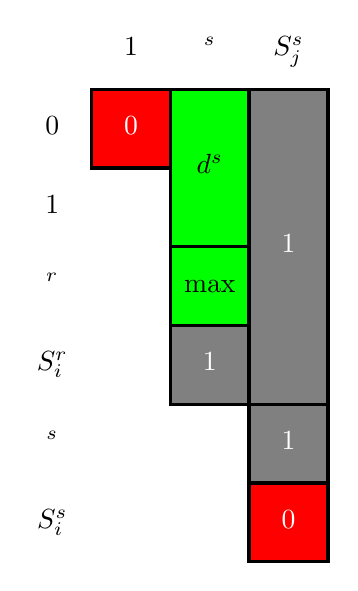
\begin{tikzpicture}[anchor=mid,rule/.style={draw=black,very thick}]
              \node at (1.5, -0.5) {\(1\)};
              \node at (2.5, -0.5) {\(\MM^s\)};
              \node at (3.5, -0.5) {\(S^s_j\)};
              \node at (0.5, -1.5) {\(0\)};
              \node at (0.5, -2.5) {\(1\)};
              \node at (0.5, -3.5) {\(\MM^r\)};
              \node at (0.5, -4.5) {\(S^r_i\)};
              \node at (0.5, -5.5) {\(\MM^s\)};
              \node at (0.5, -6.5) {\(S^s_i\)};
              \path[rule,fill=gray] (3, -1) rectangle +(1, -4);
              \path[rule,fill=gray] (3, -5) rectangle +(1, -1);
              \path[rule,fill=gray] (2, -4) rectangle +(1, -1);
              \path[rule,fill=red] (1, -1) rectangle +(1, -1);
              \path[rule,fill=red] (3, -6) rectangle +(1, -1);
              \path[rule,fill=green] (2, -1) rectangle +(1, -2);
              \path[rule,fill=green] (2, -3) rectangle +(1, -1);
              \node[text=white] at (1.5, -1.5) {0};
              \node at (2.5, -2) {\(d^s\)};
              \node at (2.5, -3.5) {\(\max\)};
              \node[text=white] at (2.5, -4.5) {1};
              \node[text=white] at (3.5, -3) {1};
              \node[text=white] at (3.5, -5.5) {1};
              \node[text=white] at (3.5, -6.5) {0};
          \end{tikzpicture}
      }{
          \caption{Block cipher plaintext collision cases (\(\mathcal{D}\))}\label{domaincollision}
      }
      \ffigbox{
          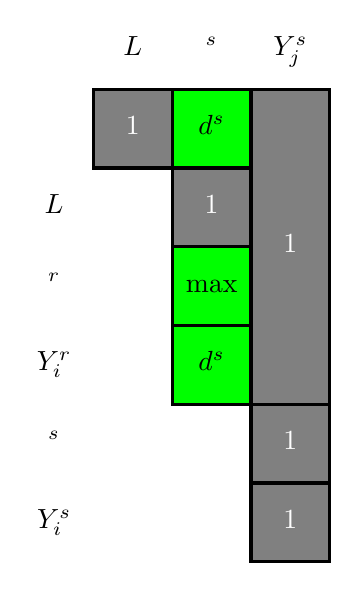
\begin{tikzpicture}[anchor=mid,rule/.style={draw=black,very thick}]
              \node at (1.5, -0.5) {\(L\)};
              \node at (2.5, -0.5) {\(\UU^s\)};
              \node at (3.5, -0.5) {\(Y^s_j\)};
              \node at (0.5, -1.5) {\(\hgen\)};
              \node at (0.5, -2.5) {\(L\)};
              \node at (0.5, -3.5) {\(\UU^r\)};
              \node at (0.5, -4.5) {\(Y^r_i\)};
              \node at (0.5, -5.5) {\(\UU^s\)};
              \node at (0.5, -6.5) {\(Y^s_i\)};
              \path[rule,fill=gray] (1, -1) rectangle +(1, -1);
              \path[rule,fill=gray] (3, -1) rectangle +(1, -4);
              \path[rule,fill=gray] (3, -5) rectangle +(1, -1);
              \path[rule,fill=gray] (3, -6) rectangle +(1, -1);
              \path[rule,fill=gray] (2, -2) rectangle +(1, -1);
              \path[rule,fill=green] (2, -3) rectangle +(1, -1);
              \path[rule,fill=green] (2, -4) rectangle +(1, -1);
              \path[rule,fill=green] (2, -1) rectangle +(1, -1);
              \node[text=white] at (1.5, -1.5) {1};
              \node at (2.5, -1.5) {\(d^s\)};
              \node[text=white] at (2.5, -2.5) {1};
              \node at (2.5, -3.5) {\(\max\)};
              \node at (2.5, -4.5) {\(d^s\)};
              \node[text=white] at (3.5, -3) {1};
              \node[text=white] at (3.5, -5.5) {1};
              \node[text=white] at (3.5, -6.5) {1};
          \end{tikzpicture}
      }{
          \caption{Block cipher ciphertext collision cases (\(\mathcal{R}\))}\label{rangecollision}
      }
  \end{floatrow}
\end{figure}
\end{document}
